\chapter{Reference Signals}

%---------- Overview ----------%
\section{Overview}
Reference signals are predefined signals occupying specific resource elements within the down-link time-frequency grid. The NR specification includes several types of reference signals transmitted in different ways and intended to be used for different purposes by a receiving device.
\newline
Unlike LTE, which relies heavily on always-on, cell-specific reference signals in the down-link for coherent demodulation, channel quality estimation for CSI reporting, and general time-frequency tracking, NR uses different down-link reference signals for different purposes. This allows for optimizing each of the reference signals for their specific purpose. It is also in line with the overall principle of ultra-lean transmission as the different reference signals can be transmitted only when needed. Later release of LTE took some steps in this direction, but NR can exploit this to a much larger degree as there are no legacy NR devices to cater for.
\newline
The NR reference signals include:
\begin{itemize}
    \item Demodulation reference signals (DMRS) for PDSCH are intended for channel estimation at the device as part of coherent demodulation. They are present only in the resource blocks used for PDSCH transmission. Similarly, the DMRS for PUSCH allows the gNB to coherently demodulate the PUSCH.
    \item Phase-tracking reference signals (PTRS) can be seen as an extension to DMRS for PDSCH/PUSCH and are intended for phase-noise compensation. The PT-RS is denser in time but sparser in frequency than the DM-RS, and, if configured, occurs only in combination with DMRS.
    \item CSI reference signals (CSI-RS) are downlink reference signals intended to be used by devices to acquire down-link channel-state information (CSI). Specific instances of CSI reference signals can be configured for time/frequency tracking and mobility measurements.
    \item Tracking reference signals (TRS) are sparse reference signals intended to assist the device in time and frequency tracking
    \item Sounding reference signals (SRS) are uplink reference signals transmitted by the devices and used for uplink channel-state estimation at the base stations.
\end{itemize}

The previous section assumed full knowledge of the channel characteristics at both transmitter and receiver sides, this section discusses how such knowledge is gained by focusing on two important reference signals : CSI-RS and DMRS.
\newline
The propagation channel depends on the transmit frequency. Therefore, if up-link and down-link operate on two different frequencies as is the case in FDD, there is no choice but relying on the receiver to communicate information about the channel back to the transmitter. This is the case at the bottom right.
\newline
In the case of TDD, where the up-link and down-link share the same transmit frequency, it is possible, on the other hand, to estimate the down-link channel based on measurements on up-link transmission (or the opposite). In this section we focus on the FDD transmission case.
%------------------------------%

%------------ DMRS ------------%
\section{DMRS}
The DM-RS in NR provides quite some flexibility to cater for different deployment scenarios and use cases: a front-loaded design to enable low latency, support for up to 12 orthogonal antenna ports for MIMO, transmissions duration from 2 to 14 symbols, and up to four reference-signal instances per slot to support very high-speed scenarios.
To achieve low latency, it is beneficial to locate the demodulation reference signals early in the transmission, sometimes known as front-loaded reference signals. This allows the receiver to obtain a channel estimate early and, once the channel estimate is obtained, process the received symbols on the fly without having to buffer a complete slot prior to data processing. This is essentially the same motivation as for the frequency-first mapping of data to the resource elements.
Two main time-domain structures are supported, differing in the location of the first DM-RS symbol:
\begin{itemize}
    \item Mapping type A, where the first DMRS is located in symbol 2 or 3 of the slot and the DMRS is mapped relative to the start of the slot boundary, regardless of where in the slot the actual data transmission starts. This mapping type is primarily intended for the case where the data occupy (most of) a slot. The reason for symbol 2 or 3 in the down-link is to locate the first DMRS occasion after a CORESET located at the beginning of a slot.
    \item Mapping type B, where the first DMRS is located in the first symbol of the data allocation, that is, the DMRS location is not given relative to the slot boundary but rather relative to where the data are located. This mapping is originally motivated by transmissions over a small fraction of the slot to support very low latency and other transmissions that benefit from not waiting until a slot boundary starts but can be used regardless of the transmission duration.
\end{itemize}

\begin{figure}[ht]
\centering
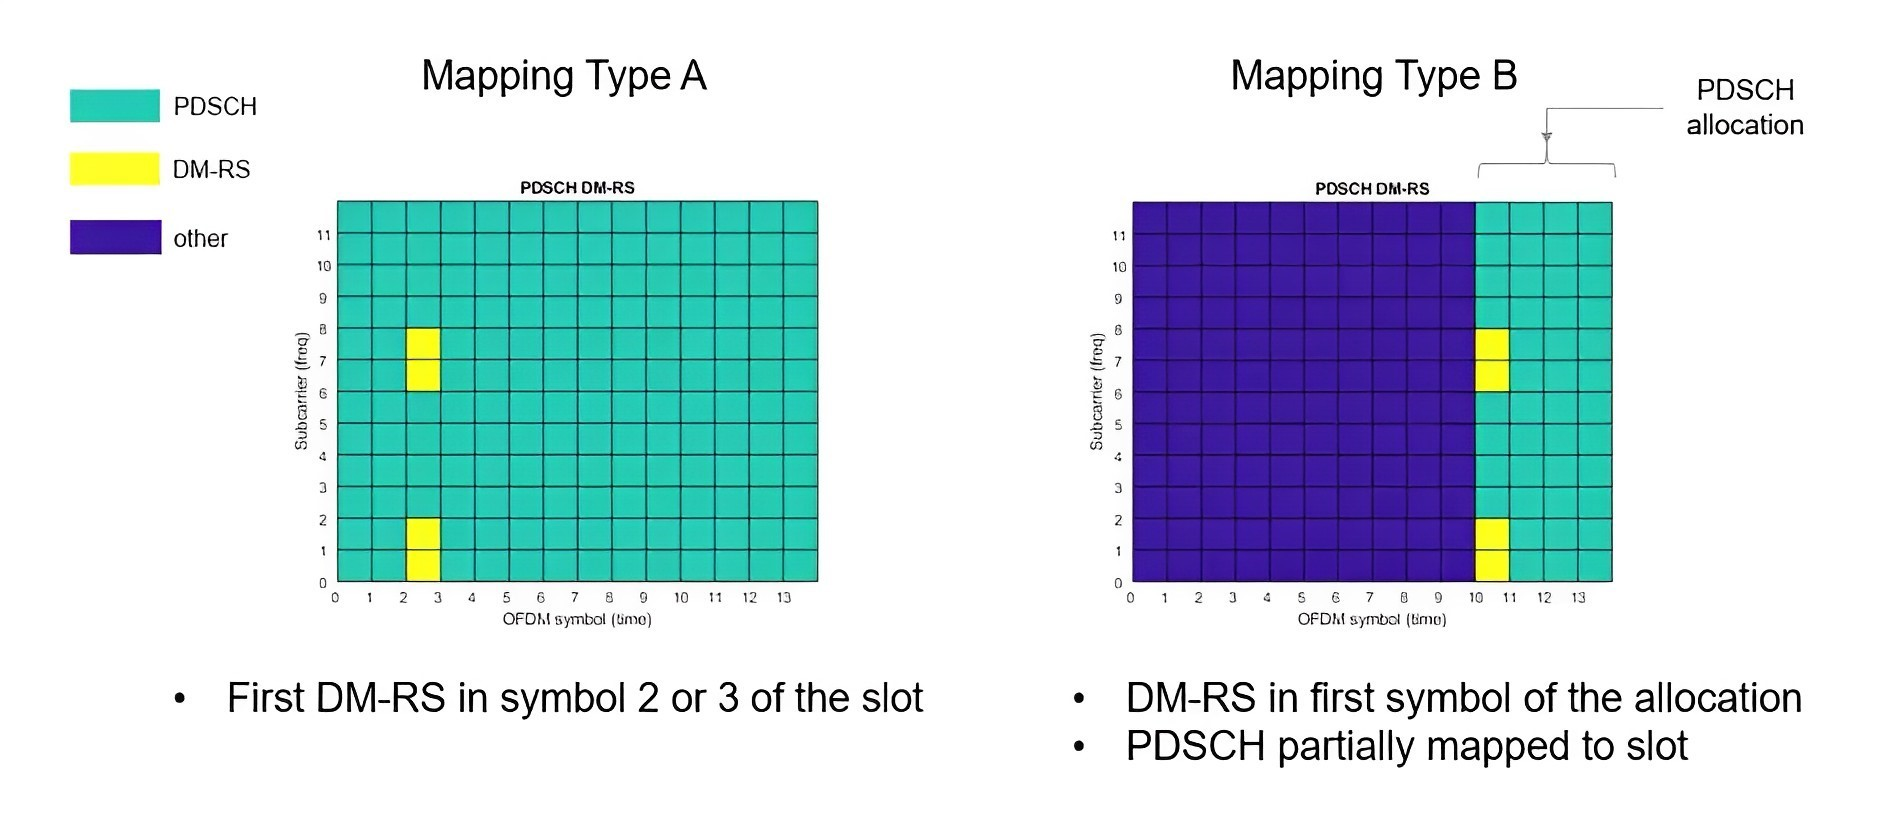
\includegraphics[width=0.6 \textwidth]{6-2.jpg}
\caption{DMRS Mapping type A \& type B }
%\label{fig:figure4.1}
\end{figure}

Although front-loaded reference signals are beneficial from a latency perspective, they may not be sufficiently dense in the time domain in the case of rapid channel variations. To support high-speed scenarios, it is possible to configure up to three additional DM-RS occasions in a slot. The channel estimator in the receiver can use these additional occasions for more accurate channel estimation, for example, to use interpolation between the occasions within a slot.

\subsection{Pilot based DMRS channel estimation}
\begin{wrapfigure}{r}{0.4\textwidth}
    \centering
    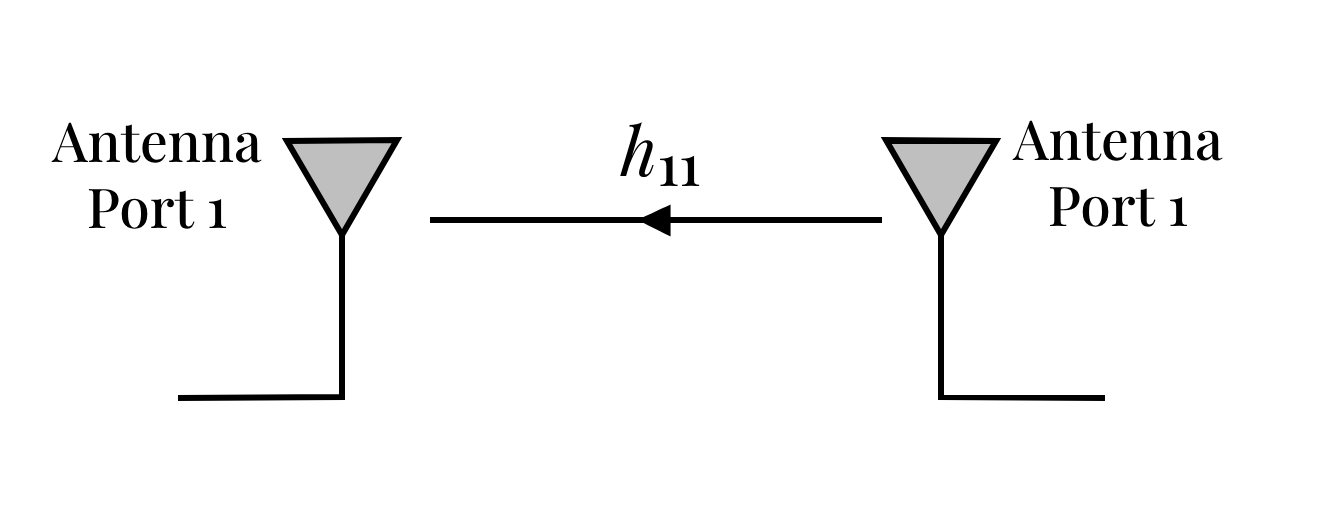
\includegraphics[width=0.4\textwidth]{7.png}
    \caption{Single Tx Single Rx}
\end{wrapfigure}

Assume a single antenna port at both Tx and Rx.
\[ y = h_{11} x \]
In order to know $h_11$, we need to send a symbol $x$ which is known at the receiver, then $h_11$ can be calculated as:
\[ h_{11} = \frac{y}{x} \]

This known symbol $x$ is called a pilot symbol.
The problem with this approach is that there exists a channel coefficient need to be known for each RE in the PDSCH which requires sending pilots in all REs, hence there will not be any place for data bits.
The solution to this problem is to send pilot symbols in some REs as shown in the figure to determine the channel coefficients in those REs.

\begin{figure}[ht]
\centering
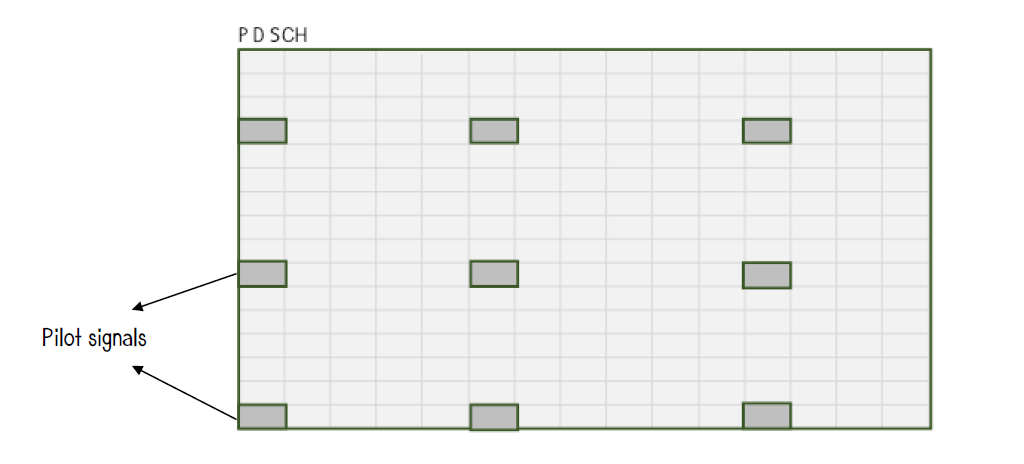
\includegraphics[width=6.47 in, height=2.36in]{8.PNG}
\caption{Pilot signals in some REs }
%\label{fig:figure4.1}
\end{figure}     

Use time/frequency correlation to determine channel coefficients in other REs

\begin{figure}[ht]
\centering
    \begin{subfigure}[b]{0.4\textwidth}
        \centering
        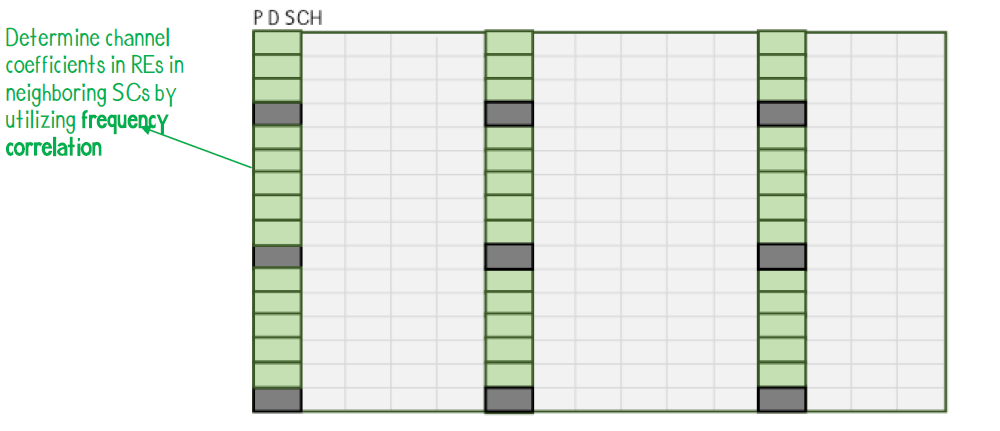
\includegraphics[width=\textwidth]{9.PNG}
        \caption{Frequency correlation }
    \end{subfigure}
    \hfill
    \begin{subfigure}[b]{0.4\textwidth}
        \centering
        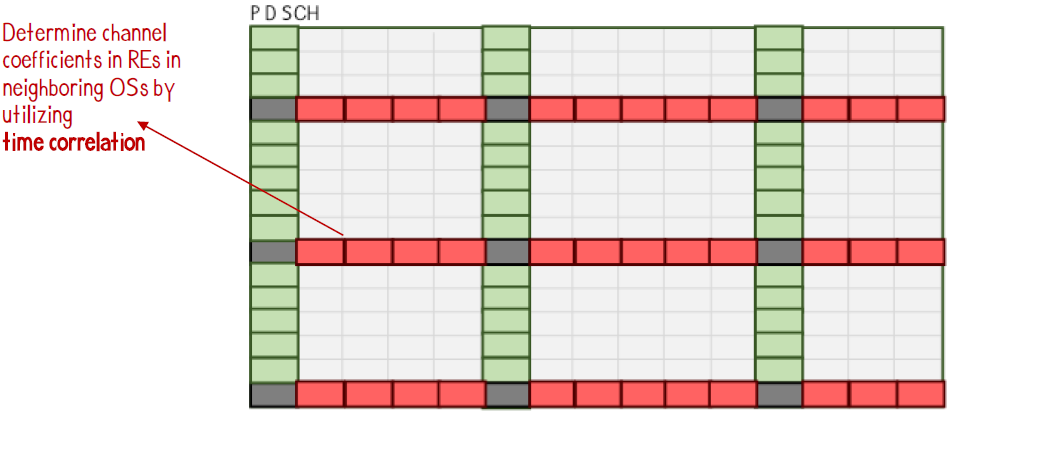
\includegraphics[width=\textwidth]{10.PNG}
        \caption{Time correlation }
    \end{subfigure}
    \hfill
    \begin{subfigure}[c]{0.4\textwidth}
        \centering
        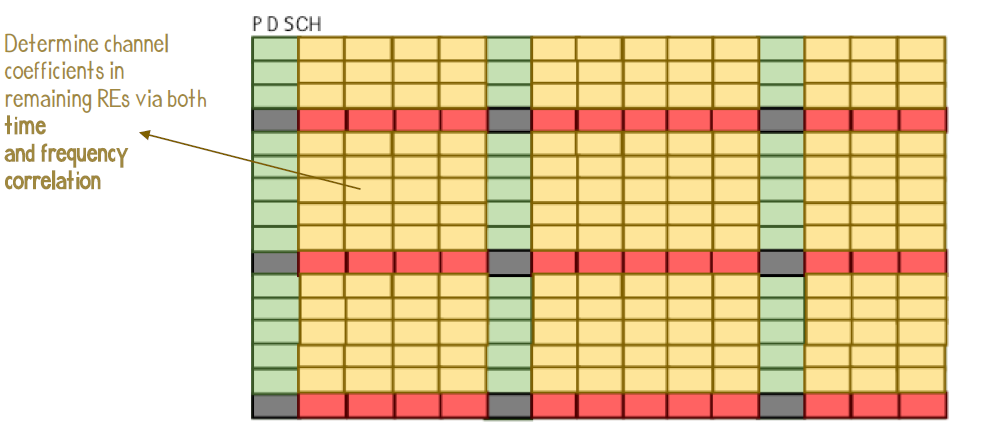
\includegraphics[width=\textwidth]{11.PNG}
        \caption{Time / frequency correlation }
    \end{subfigure}
       \caption{Correlation in time \& frequency}
\end{figure}

For the above property to be used time and frequency correlations must be determined, these are known using coherence time and coherence bandwidth.
\newline\newline
Coherence bandwidth is a statistical measurement of the range of frequencies over which the channel can be considered "flat", or in other words the approximate maximum bandwidth or frequency interval over which two frequencies of a signal are likely to experience comparable or correlated amplitude fading. If the multi-path time delay spread equals D seconds, then the coherence bandwidth $B_c$ is given approximately by the equation

\[ B_c 	\approx \frac{1}{D}  \]

Hence if the delay spread is small, frequency correlation is high which means we need less pilots density in the frequency domain.
\begin{figure}[ht]
\centering
    \begin{subfigure}[b]{0.4\textwidth}
        \centering
        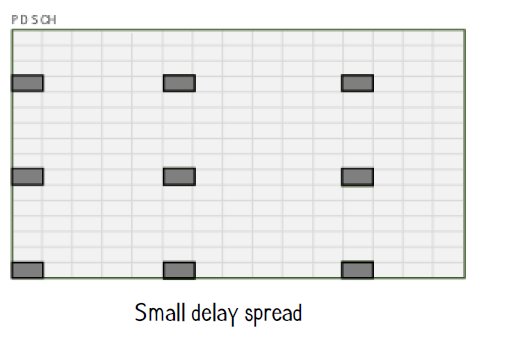
\includegraphics[width=\textwidth]{12.PNG}
        \caption{Small delay spread }
    \end{subfigure}
    \hfill
    \begin{subfigure}[b]{0.4\textwidth}
        \centering
        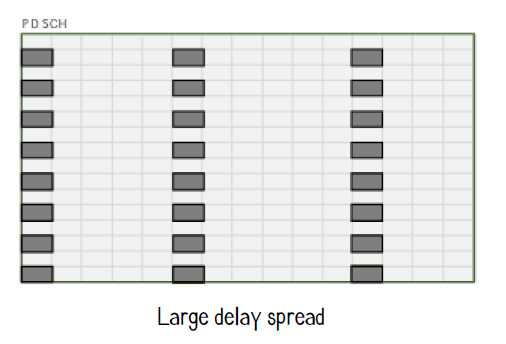
\includegraphics[width=\textwidth]{13.PNG}
        \caption{Large delay spread }
    \end{subfigure}
       \caption{Delay spread effect}
\end{figure}

Coherence time is the time duration over which the channel impulse response is considered to be not varying. Such channel variation is much more significant in wireless communications systems, due to Doppler effects. If the maximum doppler spread equals $f_m$ Hz, then the coherence time $T_c$ is given approximately by the equation
\[ T_c 	\approx \frac{1}{f_m}  \]

Hence if the doppler spread is small, time correlation is high which means we need less pilots density in the time domain.

\begin{figure}[ht]
\centering
    \begin{subfigure}[b]{0.4\textwidth}
        \centering
        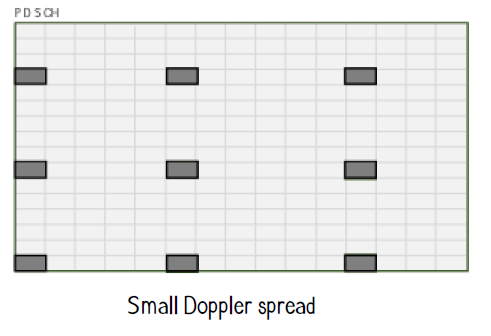
\includegraphics[width=\textwidth]{14.PNG}
        \caption{Small Doppler spread }
    \end{subfigure}
    \hfill
    \begin{subfigure}[b]{0.4\textwidth}
        \centering
        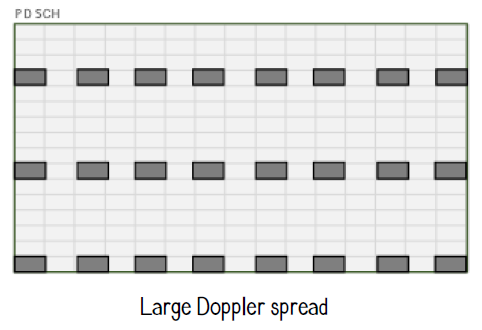
\includegraphics[width=\textwidth]{15.PNG}
        \caption{Large Doppler spread}
    \end{subfigure}
       \caption{Doppler spread effect}
\end{figure}
%-----------------------------%


\section{CSI Reference Signal}

\section{Channel Estimation}